\documentclass{standalone}
\usepackage{tikz}
\usetikzlibrary{patterns, positioning}
\usepackage[sfdefault]{ClearSans} %% option 'sfdefault' activates Clear Sans as the default text font
\usepackage[T1]{fontenc}

\begin{document}
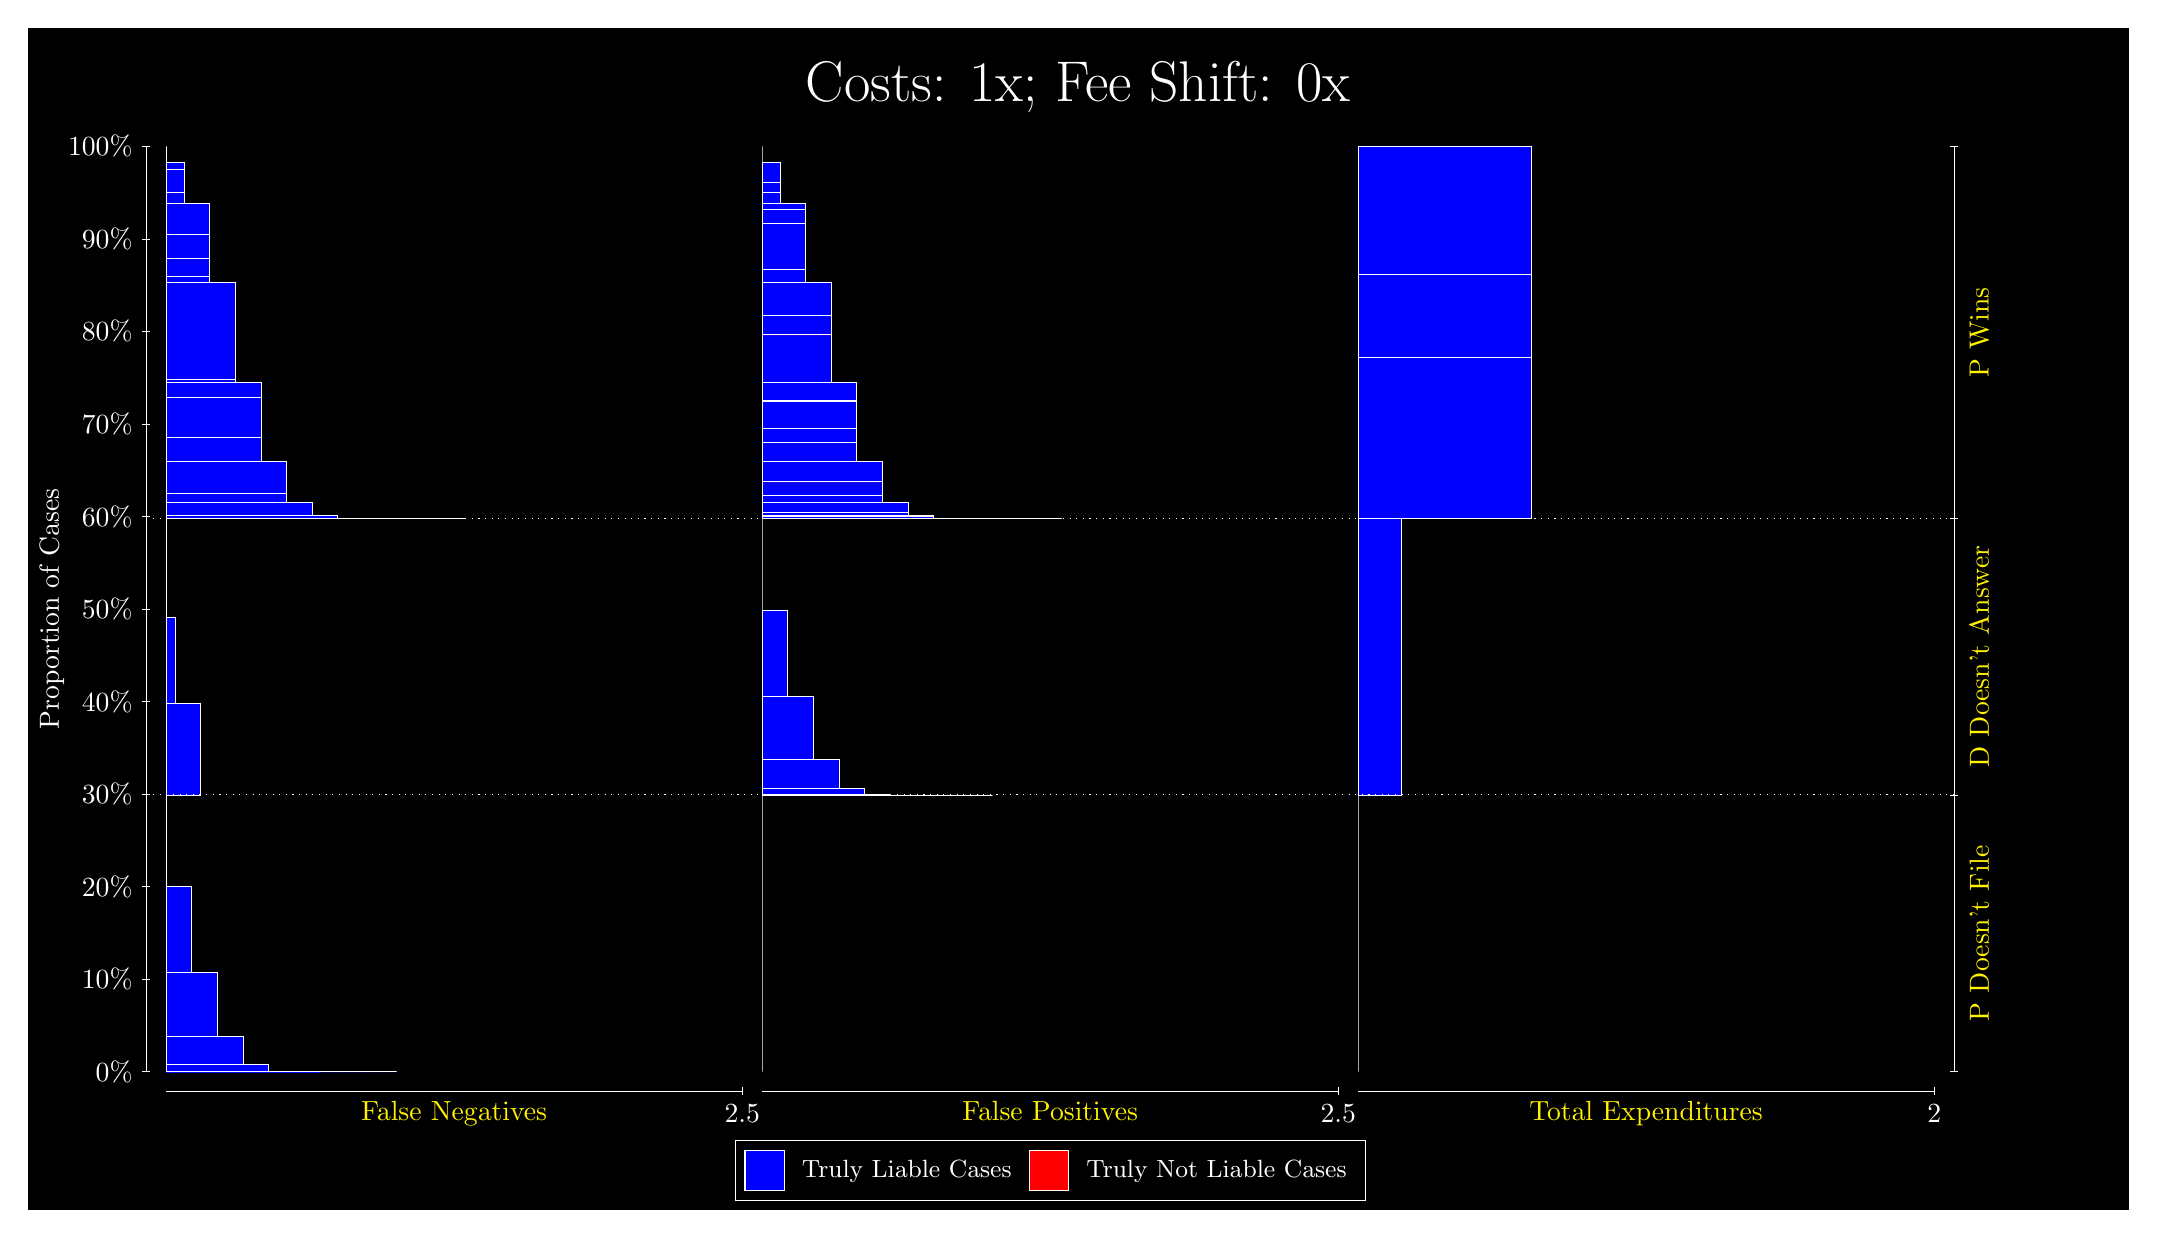
\begin{tikzpicture}
\draw[fill=black] (0,0) rectangle (26.667,15);
\draw[text=white] (0,13.5) rectangle (26.667,15) node[midway] {\huge Costs: 1x; Fee Shift: 0x};
\draw[white, very thin] (1.5,1.75) -- (1.5,13.5);
\node[rotate=90, text=white, anchor=center] at (0.3, 7.625) {Proportion of Cases};
\draw[white, very thin] (1.45,1.75) -- (1.55,1.75);
\node[text=white, anchor=east] at (1.45, 1.75) {0\%};
\draw[white, very thin] (1.45,2.925) -- (1.55,2.925);
\node[text=white, anchor=east] at (1.45, 2.925) {10\%};
\draw[white, very thin] (1.45,4.1) -- (1.55,4.1);
\node[text=white, anchor=east] at (1.45, 4.1) {20\%};
\draw[white, very thin] (1.45,5.275) -- (1.55,5.275);
\node[text=white, anchor=east] at (1.45, 5.275) {30\%};
\draw[white, very thin] (1.45,6.45) -- (1.55,6.45);
\node[text=white, anchor=east] at (1.45, 6.45) {40\%};
\draw[white, very thin] (1.45,7.625) -- (1.55,7.625);
\node[text=white, anchor=east] at (1.45, 7.625) {50\%};
\draw[white, very thin] (1.45,8.8) -- (1.55,8.8);
\node[text=white, anchor=east] at (1.45, 8.8) {60\%};
\draw[white, very thin] (1.45,9.975) -- (1.55,9.975);
\node[text=white, anchor=east] at (1.45, 9.975) {70\%};
\draw[white, very thin] (1.45,11.15) -- (1.55,11.15);
\node[text=white, anchor=east] at (1.45, 11.15) {80\%};
\draw[white, very thin] (1.45,12.325) -- (1.55,12.325);
\node[text=white, anchor=east] at (1.45, 12.325) {90\%};
\draw[white, very thin] (1.45,13.5) -- (1.55,13.5);
\node[text=white, anchor=east] at (1.45, 13.5) {100\%};

\draw[white, very thin] (24.457,1.75) -- (24.457,13.5);
\draw[white, very thin] (24.407,1.75) -- (24.507,1.75);
\node[anchor=west] at (24.407, 1.75) {};
\draw[white, very thin] (24.407,5.264) -- (24.507,5.264);
\node[anchor=west] at (24.407, 5.264) {};
\draw[white, very thin] (24.407,8.7768) -- (24.507,8.7768);
\node[anchor=west] at (24.407, 8.7768) {};
\draw[white, very thin] (24.407,13.5) -- (24.507,13.5);
\node[anchor=west] at (24.407, 13.5) {};

\draw[white, very thin, fill=blue] (1.75,1.75) rectangle (4.6775,1.75);
\draw[white, very thin, fill=blue] (1.75,1.75) rectangle (4.3523,1.75);
\draw[white, very thin, fill=blue] (1.75,1.75) rectangle (4.027,1.75);
\draw[white, very thin, fill=blue] (1.75,1.75) rectangle (3.7017,1.7503);
\draw[white, very thin, fill=blue] (1.75,1.7503) rectangle (3.3764,1.7576);
\draw[white, very thin, fill=blue] (1.75,1.7576) rectangle (3.0511,1.8361);
\draw[white, very thin, fill=blue] (1.75,1.8361) rectangle (2.7258,2.1984);
\draw[white, very thin, fill=blue] (1.75,2.1984) rectangle (2.4006,3.0086);
\draw[white, very thin, fill=blue] (1.75,3.0086) rectangle (2.0753,4.0995);
\draw[white, very thin, fill=red] (1.75,4.0995) rectangle (1.75,4.0995);
\draw[white, very thin, fill=blue] (1.75,4.0995) rectangle (1.75,5.264);
\draw[white, very thin, fill=blue] (1.75,5.264) rectangle (2.1891,6.4284);
\draw[white, very thin, fill=blue] (1.75,6.4284) rectangle (1.8638,7.5193);
\draw[white, very thin, fill=red] (1.75,7.5193) rectangle (1.75,7.5193);
\draw[white, very thin, fill=blue] (1.75,7.5193) rectangle (1.75,8.7768);
\draw[white, very thin, fill=blue] (1.75,8.7768) rectangle (5.5558,8.7768);
\draw[white, very thin, fill=blue] (1.75,8.7768) rectangle (5.2305,8.7768);
\draw[white, very thin, fill=blue] (1.75,8.7768) rectangle (4.9052,8.7768);
\draw[white, very thin, fill=blue] (1.75,8.7768) rectangle (4.58,8.7768);
\draw[white, very thin, fill=blue] (1.75,8.7768) rectangle (4.58,8.7769);
\draw[white, very thin, fill=blue] (1.75,8.7769) rectangle (4.2547,8.7788);
\draw[white, very thin, fill=blue] (1.75,8.7788) rectangle (4.2547,8.7799);
\draw[white, very thin, fill=blue] (1.75,8.7799) rectangle (3.9294,8.8095);
\draw[white, very thin, fill=blue] (1.75,8.8095) rectangle (3.6041,8.9737);
\draw[white, very thin, fill=blue] (1.75,8.9737) rectangle (3.2788,9.0947);
\draw[white, very thin, fill=blue] (1.75,9.0947) rectangle (3.2788,9.4955);
\draw[white, very thin, fill=blue] (1.75,9.4955) rectangle (2.9535,9.499);
\draw[white, very thin, fill=blue] (1.75,9.499) rectangle (2.9535,9.8098);
\draw[white, very thin, fill=blue] (1.75,9.8098) rectangle (2.9535,10.315);
\draw[white, very thin, fill=blue] (1.75,10.315) rectangle (2.9535,10.509);
\draw[white, very thin, fill=blue] (1.75,10.509) rectangle (2.6283,10.539);
\draw[white, very thin, fill=blue] (1.75,10.539) rectangle (2.6283,11.768);
\draw[white, very thin, fill=blue] (1.75,11.768) rectangle (2.303,11.849);
\draw[white, very thin, fill=blue] (1.75,11.849) rectangle (2.303,12.079);
\draw[white, very thin, fill=blue] (1.75,12.079) rectangle (2.303,12.378);
\draw[white, very thin, fill=blue] (1.75,12.378) rectangle (2.303,12.781);
\draw[white, very thin, fill=blue] (1.75,12.781) rectangle (1.9777,12.915);
\draw[white, very thin, fill=blue] (1.75,12.915) rectangle (1.9777,13.212);
\draw[white, very thin, fill=blue] (1.75,13.212) rectangle (1.9777,13.303);
\draw[white, very thin, fill=red] (1.75,13.303) rectangle (1.75,13.303);
\draw[white, very thin, fill=blue] (1.75,13.303) rectangle (1.75,13.5);
\draw[white, very thin, fill=red] (9.3189,1.75) rectangle (9.3189,1.75);
\draw[white, very thin, fill=blue] (9.3189,1.75) rectangle (9.3189,5.264);
\draw[white, very thin, fill=red] (9.3189,5.264) rectangle (12.246,5.264);
\draw[white, very thin, fill=blue] (9.3189,5.264) rectangle (12.246,5.264);
\draw[white, very thin, fill=blue] (9.3189,5.264) rectangle (11.921,5.264);
\draw[white, very thin, fill=blue] (9.3189,5.264) rectangle (11.596,5.264);
\draw[white, very thin, fill=blue] (9.3189,5.264) rectangle (11.271,5.2641);
\draw[white, very thin, fill=blue] (9.3189,5.2641) rectangle (10.945,5.271);
\draw[white, very thin, fill=blue] (9.3189,5.271) rectangle (10.62,5.349);
\draw[white, very thin, fill=blue] (9.3189,5.349) rectangle (10.295,5.7112);
\draw[white, very thin, fill=blue] (9.3189,5.7112) rectangle (9.9694,6.5214);
\draw[white, very thin, fill=blue] (9.3189,6.5214) rectangle (9.6442,7.6123);
\draw[white, very thin, fill=blue] (9.3189,7.6123) rectangle (9.3189,8.7768);
\draw[white, very thin, fill=red] (9.3189,8.7768) rectangle (13.125,8.7768);
\draw[white, very thin, fill=blue] (9.3189,8.7768) rectangle (13.125,8.7768);
\draw[white, very thin, fill=red] (9.3189,8.7768) rectangle (12.799,8.7768);
\draw[white, very thin, fill=blue] (9.3189,8.7768) rectangle (12.799,8.7768);
\draw[white, very thin, fill=blue] (9.3189,8.7768) rectangle (12.474,8.7768);
\draw[white, very thin, fill=red] (9.3189,8.7768) rectangle (12.474,8.7768);
\draw[white, very thin, fill=blue] (9.3189,8.7768) rectangle (12.474,8.7768);
\draw[white, very thin, fill=blue] (9.3189,8.7768) rectangle (12.149,8.7769);
\draw[white, very thin, fill=blue] (9.3189,8.7769) rectangle (12.149,8.7769);
\draw[white, very thin, fill=red] (9.3189,8.7769) rectangle (12.149,8.7769);
\draw[white, very thin, fill=blue] (9.3189,8.7769) rectangle (12.149,8.7769);
\draw[white, very thin, fill=red] (9.3189,8.7769) rectangle (11.824,8.7769);
\draw[white, very thin, fill=blue] (9.3189,8.7769) rectangle (11.824,8.7793);
\draw[white, very thin, fill=blue] (9.3189,8.7793) rectangle (11.824,8.7798);
\draw[white, very thin, fill=blue] (9.3189,8.7798) rectangle (11.824,8.7799);
\draw[white, very thin, fill=red] (9.3189,8.7799) rectangle (11.498,8.7799);
\draw[white, very thin, fill=blue] (9.3189,8.7799) rectangle (11.498,8.8063);
\draw[white, very thin, fill=blue] (9.3189,8.8063) rectangle (11.498,8.8095);
\draw[white, very thin, fill=blue] (9.3189,8.8095) rectangle (11.173,8.8553);
\draw[white, very thin, fill=red] (9.3189,8.8553) rectangle (11.173,8.8553);
\draw[white, very thin, fill=blue] (9.3189,8.8553) rectangle (11.173,8.9737);
\draw[white, very thin, fill=blue] (9.3189,8.9737) rectangle (10.848,9.0647);
\draw[white, very thin, fill=blue] (9.3189,9.0647) rectangle (10.848,9.2406);
\draw[white, very thin, fill=red] (9.3189,9.2406) rectangle (10.848,9.2406);
\draw[white, very thin, fill=blue] (9.3189,9.2406) rectangle (10.848,9.4955);
\draw[white, very thin, fill=blue] (9.3189,9.4955) rectangle (10.522,9.7466);
\draw[white, very thin, fill=blue] (9.3189,9.7466) rectangle (10.522,9.9196);
\draw[white, very thin, fill=red] (9.3189,9.9196) rectangle (10.522,9.9196);
\draw[white, very thin, fill=blue] (9.3189,9.9196) rectangle (10.522,10.258);
\draw[white, very thin, fill=blue] (9.3189,10.258) rectangle (10.522,10.279);
\draw[white, very thin, fill=blue] (9.3189,10.279) rectangle (10.522,10.509);
\draw[white, very thin, fill=blue] (9.3189,10.509) rectangle (10.197,11.109);
\draw[white, very thin, fill=red] (9.3189,11.109) rectangle (10.197,11.109);
\draw[white, very thin, fill=blue] (9.3189,11.109) rectangle (10.197,11.354);
\draw[white, very thin, fill=blue] (9.3189,11.354) rectangle (10.197,11.768);
\draw[white, very thin, fill=blue] (9.3189,11.768) rectangle (9.8718,11.941);
\draw[white, very thin, fill=blue] (9.3189,11.941) rectangle (9.8718,12.528);
\draw[white, very thin, fill=blue] (9.3189,12.528) rectangle (9.8718,12.701);
\draw[white, very thin, fill=blue] (9.3189,12.701) rectangle (9.8718,12.781);
\draw[white, very thin, fill=blue] (9.3189,12.781) rectangle (9.5466,12.915);
\draw[white, very thin, fill=blue] (9.3189,12.915) rectangle (9.5466,13.048);
\draw[white, very thin, fill=blue] (9.3189,13.048) rectangle (9.5466,13.303);
\draw[white, very thin, fill=blue] (9.3189,13.303) rectangle (9.3189,13.5);
\draw[white, very thin, fill=red] (16.888,1.75) rectangle (16.888,1.75);
\draw[white, very thin, fill=blue] (16.888,1.75) rectangle (16.888,5.264);
\draw[white, very thin, fill=red] (16.888,5.264) rectangle (17.437,5.264);
\draw[white, very thin, fill=blue] (16.888,5.264) rectangle (17.437,8.7768);
\draw[white, very thin, fill=red] (16.888,8.7768) rectangle (19.083,8.7768);
\draw[white, very thin, fill=blue] (16.888,8.7768) rectangle (19.083,10.821);
\draw[white, very thin, fill=red] (16.888,10.821) rectangle (19.083,10.821);
\draw[white, very thin, fill=blue] (16.888,10.821) rectangle (19.083,11.876);
\draw[white, very thin, fill=red] (16.888,11.876) rectangle (19.083,11.876);
\draw[white, very thin, fill=blue] (16.888,11.876) rectangle (19.083,13.5);
\draw[white, dotted] (1.5,5.264) -- (24.457,5.264);
\draw[white, dotted] (1.5,8.7768) -- (24.457,8.7768);
\draw[white, very thin] (1.75,1.5) -- (9.0689,1.5);
\node[text=yellow, anchor=north] at (5.4094, 1.5) {False Negatives};
\draw[white, very thin] (9.0689,1.45) -- (9.0689,1.55);
\node[text=white, anchor=north] at (9.0689, 1.45) {2.5};

\draw[white, very thin] (9.3189,1.5) -- (16.638,1.5);
\node[text=yellow, anchor=north] at (12.978, 1.5) {False Positives};
\draw[white, very thin] (16.638,1.45) -- (16.638,1.55);
\node[text=white, anchor=north] at (16.638, 1.45) {2.5};

\draw[white, very thin] (16.888,1.5) -- (24.207,1.5);
\node[text=yellow, anchor=north] at (20.547, 1.5) {Total Expenditures};
\draw[white, very thin] (24.207,1.45) -- (24.207,1.55);
\node[text=white, anchor=north] at (24.207, 1.45) {2};

\node[text=yellow, centered, rotate=90] at (24.777, 3.507) {P Doesn't File};
\node[text=yellow, centered, rotate=90] at (24.777, 7.0204) {D Doesn't Answer};
\node[text=yellow, centered, rotate=90] at (24.777, 11.138) {P Wins};

\draw (12.978300999999998,1.5) node[draw=none] (baseCoordinate) {};
\begin{scope}[align=center]
        \matrix[scale=0.5, draw=white, below=0.5cm of baseCoordinate, nodes={draw}, column sep=0.1cm]{
            \node[rectangle, draw, minimum width=0.5cm, minimum height=0.5cm, fill=blue] {}; &
            \node[draw=none, font=\small, text=white] (B) {Truly Liable Cases}; &
            \node[rectangle, draw, minimum width=0.5cm, minimum height=0.5cm, fill=red] {}; &
            \node[draw=none, font=\small, text=white] (B) {Truly Not Liable Cases}; \\
            };
\end{scope}

\end{tikzpicture}
\end{document}